% !TeX root =../main.tex
\chapter{Implementation and Validation of the Inductor in LTspice} \label{sec:cha4}
In this chapter, the measurements of the previous chapter are used to create a simulated inductor model in LTspice. The goal: create a mixture of these to best recreate the reality of the inductor's behaviour. Again, three different approaches are taken, each mapping directly to one of the phenomena measured in chapter \ref{sec:cha3}. In each case, the used model is introduced first, followed by the steps taken to include the measured data in the model. The models are then separately simulated in different configurations and validated using available data. 

\section{Modeling the Frequency Response of the Inductor} \label{sec:modeling_the_frequency_response_of_the_inductor}
The first and simplest type of inserting non-idealities into the inductor Model of LTspice is with an \ac{ECM}. It can simulate the frequency response of a real inductor. The base inductor already has an \ac{ECM} pictured in figure \ref{fig:inductor_ecm}, taking into account the equivalent parallel capacitance between the individual windings of the inductor $EPC$, the copper resistance at low frequencies $ESR$ and the overall resistance during resonance $EPR$. It acts as a starting point to approximate the frequency response of an inductor and as later demonstrated, is enough to characterise the studied inductor's frequency response fully.
\begin{figure}[H]
    \centering
    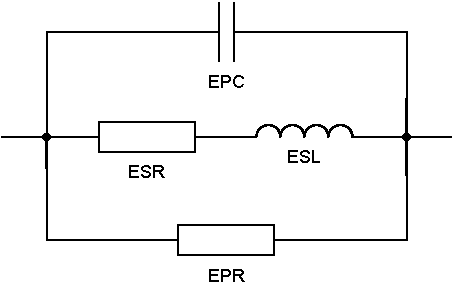
\includegraphics[width=0.5\linewidth]{Bilder//Kapitel3/Inductor_ECM.pdf}
    \caption{Inductor \ac{ECM}}
    \label{fig:inductor_ecm}
\end{figure}
Using the resulting graphs of section \ref{sec:the_frequency_response_of_the_inductor}, all four parameters of the \ac{ECM} can quickly be determined. The series resistance is equal to the magnitude of the impedance at its lowest frequency. Even though the phase at this point still isn't zero and therefore inductive properties remain, the approximation still holds true, as both magnitude and phase level out before this point. The inductance is determined similarly and can be read from the series inductance graph for low frequencies. Parallel capacitance and resistance are determined by the point of resonance. For the \textit{SER1512-223ME} inductor, the resonant point lies at \SI{14,725}{\mega\Hz} with a pure resistance of \SI{5,582}{\kilo$\Omega$}. This resistance defines the parallel resistance of the \ac{ECM}. For the parallel capacitance, the point of resonance is used, as the inductive reactance and capacitive reactance are equal in magnitude. Rearranging this equation, the capacitance can be determined by
\begin{equation}\label{eq:ecm_capacitance}
    C_P = \frac{1}{\left(2 \pi \cdot f_r\right)^2\cdot L} \quad\text{\cite{bitschnauPowerInductorModelling}.}
\end{equation}
Simulating the frequency response in LTspice is done by connecting the inductor model to a current source set to \ac{AC} analysis, mirroring the operation of the "Bode 100". The current source sweeps the chosen frequency range with a sinusoidal current with an amplitude of \SI{1}{A}. Measuring the voltage across the entire equivalent circuit after running an \ac{AC} simulation yields the frequency response of the inductor. Since the amplitude and phase of the voltage are determined by the product of the frequency-dependent impedance and the current, which is always \SI{1}{A} with a \SI{0}{\degree} angle, the complex measured voltage value equals the responding impedance value $Z_L$ at that frequency. The \ac{Q-factor} gives insight into how well the inductor is approximating an ideal inductor, showing a range for the optimal operating frequency for the inductor considering pure sinusoidal excitation. It is calculated by
\begin{equation}
    Q = \frac{Im(Z_L)}{Re(Z_L)} \quad\text{.} 
\end{equation}
The inductance simply is the imaginary part of the impedance, divided by the angular frequency up until resonance, as after that the inductor behaves like a capacitor. 
\begin{figure}[H]
    \begin{subfigure}[b]{0.50\textwidth}
        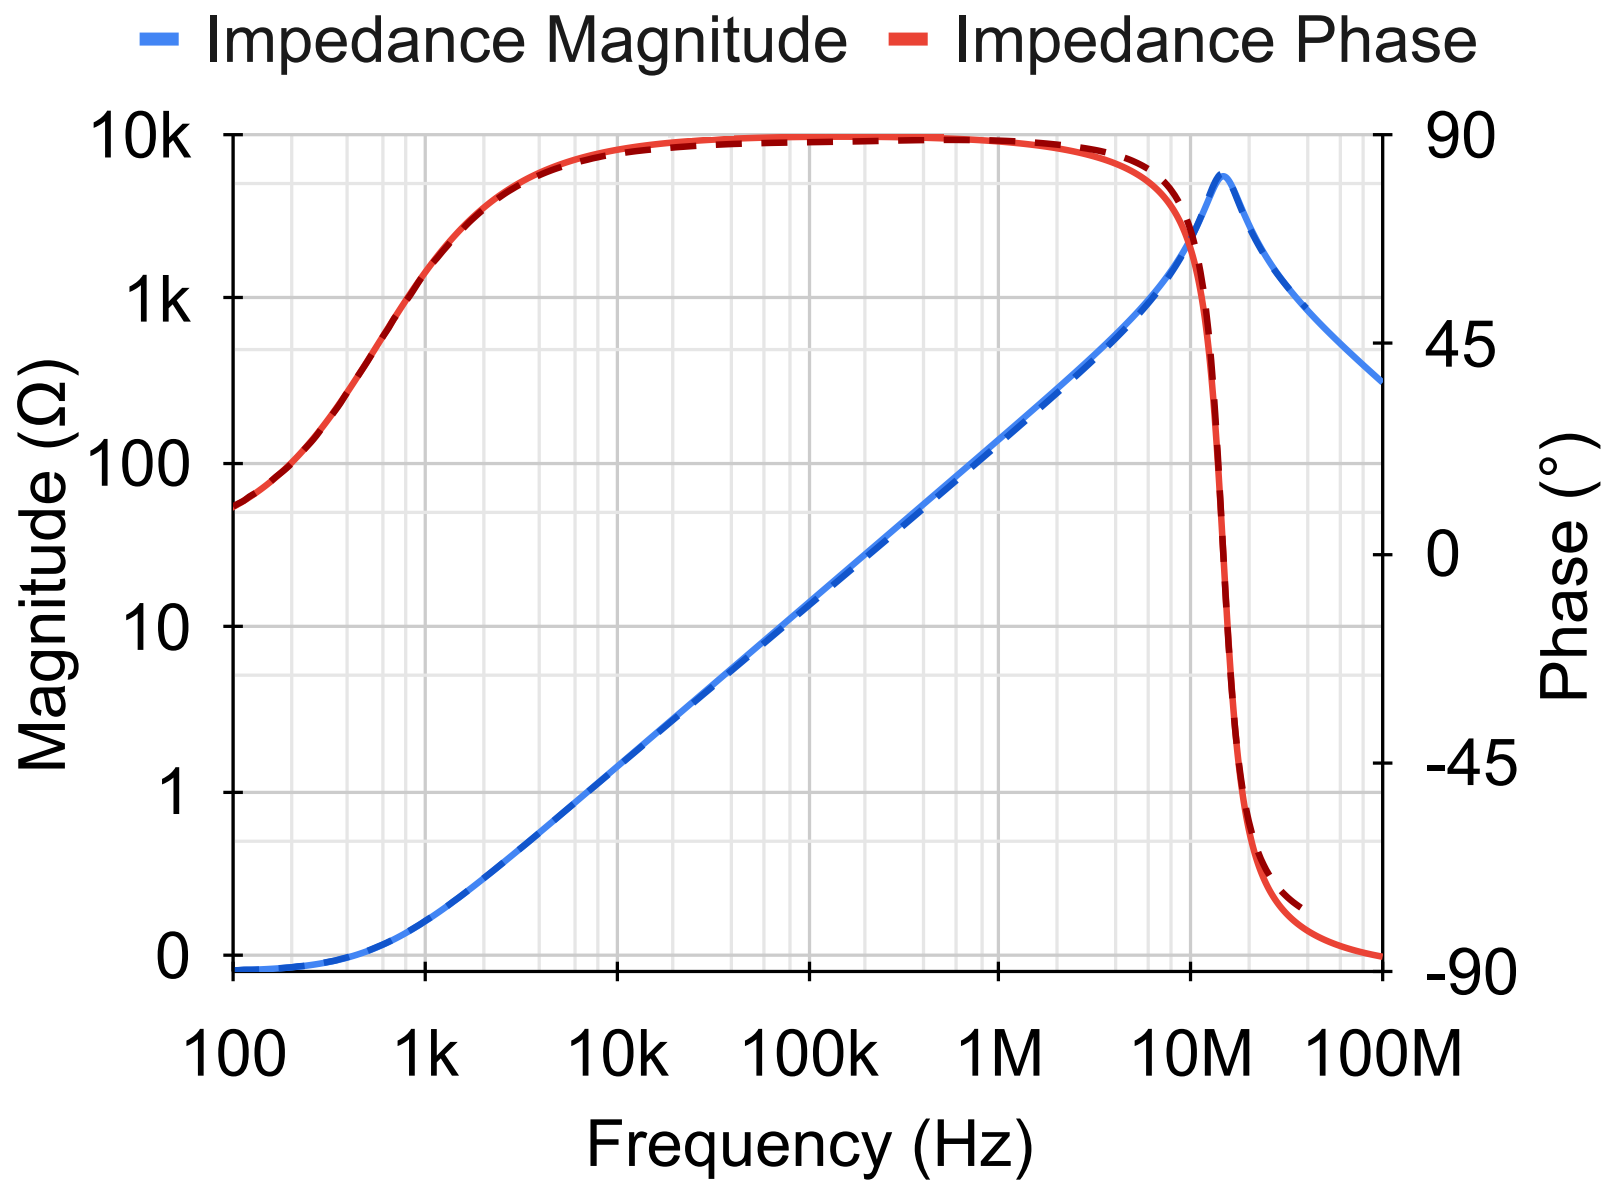
\includegraphics[width=\textwidth]{Bilder/Kapitel3/SER223_BodePlot_Combined.png}
        \caption{SER1512-223ME complex magnitude and phase vs frequency}
    \end{subfigure}
    \begin{subfigure}[b]{0.50\textwidth}
        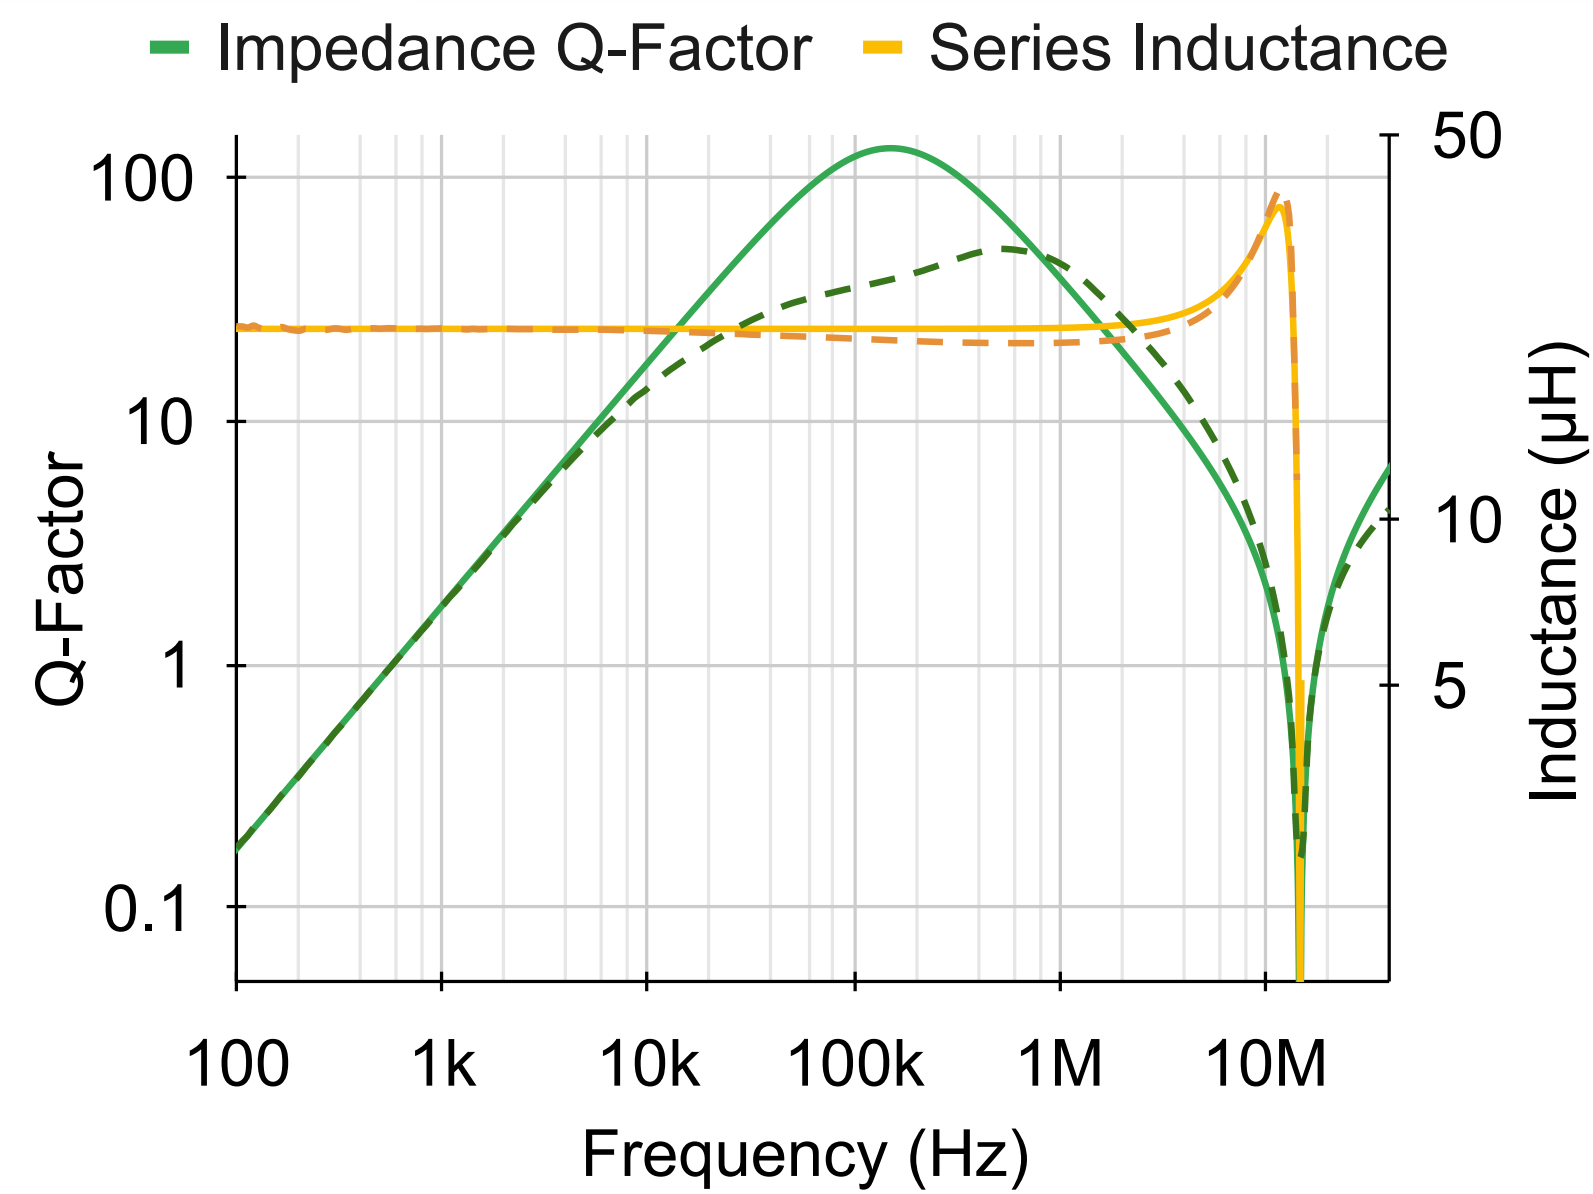
\includegraphics[width=\textwidth]{Bilder/Kapitel3/SER223_QLPlot_Combined.png}
        \caption{SER1512-223ME \ac{Q-factor} and inductance vs frequency}
    \end{subfigure}
    \caption{Simulated and measured frequency response of the SER1512-223ME\\striped lines indicate measured values, while continuous lines are simulated}
    \label{fig:bode_100_measurements_combined}							
\end{figure}
Overlaying the results of the measurements and the LTspice simulation in figure \ref{fig:bode_100_measurements_combined}, the \ac{ECM} closely models the true frequency response, justifying its use. While impedance magnitude and phase match close to perfectly, the \ac{Q-factor} and inductance slightly stray from the true values. Since the \ac{Q-factor} is sensitive to small changes in the imaginary part of the impedance its deviation from the measurement can be attributed to the slight frequency dependence of the measured inductance. The small change of the inductance before resonance is not separately modelled in the simulation \ac{ECM}, leading to the error in the \ac{Q-factor}.
Using this approach, all five inductors were modelled and implemented in LTspice with similar results to the ones presented. The results of figure \ref{fig:bode_100_measurements} show, that the frequency response of the simulated inductor is able to fully recreate the frequency behaviour of the physical inductor.

\section{Modeling the Saturation Behaviour of the Inductor}\label{sec:modeling_the_saturation_behaviour_of_the_inductor}
The second type of inductor loss modelling takes advantage of the LTspice inbuilt \textit{flux} function. With it, a specific saturation curve can be input into the inductor, modelling the current dependence of the inductance. Since this model does not influence the frequency behaviour of the inductor, it is used in combination with the results from the previous section, only replacing the inductor of the \ac{ECM} by the \textit{flux} function.\\
The validation of the model takes place in two steps. To start with, the saturation measurement is recreated in LTspice to measure the simulated saturation curve. Following this, the model is subjected to the excitation of a buck converter where the ripple current's amplitude $\Delta I_{L_r}$ is compared for different \ac{DC} biases. 

To represent the current behaviour of the inductance in the simulation, the measured data needs to be imported. Directly importing the measured flux from section \ref{sec:the_saturation_behaviour_of_the_inductor} value by value into LTspice is no option, as both the number of values LTspice able to be stored is limited and the runtime of the simulation is drastically increased. Instead, curves are fitted to the saturation measurements that best describe the inductance for each inductor. A combination of different degree polynomials and exponential functions define a piecewise function that approximates the saturation behaviour of the inductance. Integrating this function yields the flux curve, which can then be imported into LTspice using the \textit{flux}-command of the inductor.

\subsection{Validation by Saturation Behaviour}\label{sec:validation_by_saturation}
Measuring the inductance curve in the simulation is done by subjecting the inductor to an \ac{AC} with an amplitude of $\frac{1}{2\pi}$\SI{ }{\A}, frequency of \SI{1}{\Hz} and a varying \ac{DC} offset. The chosen values enable the inductance to be determined by measuring the voltage across the inductor. As the inductor's voltage is the product of the \ac{AC} amplitude and the inductor's complex impedance, the frequency factor of $2\pi$ and the current's amplitude cancel out, resulting in the voltage being numerically equivalent to the inductance.
\begin{equation}\label{eq:inductance_from_voltage}
    \hat{V}_L = \hat{I}_L \cdot j 2\pi f\cdot L \triangleq L
\end{equation}
Comparing the inductance curve of the \textit{UA8014-AL} inductor when measured and simulated, the flexibility and precision of this approach can be well demonstrated. The fitted curve, consisting of many piecewise-defined functions, is able to closely follow the measured inductance. While sensibly extending the inductance curve for values close to \SI{0}{\A} of current, high-frequency measurement noise is also removed, visible in the low amperage range of the measured inductance curve. Furthermore, it has the advantage of causing no noticeable increase to the simulation runtime when compared to a model without the \textit{flux}-command utilised. 
\begin{figure}[H]
    \centering
    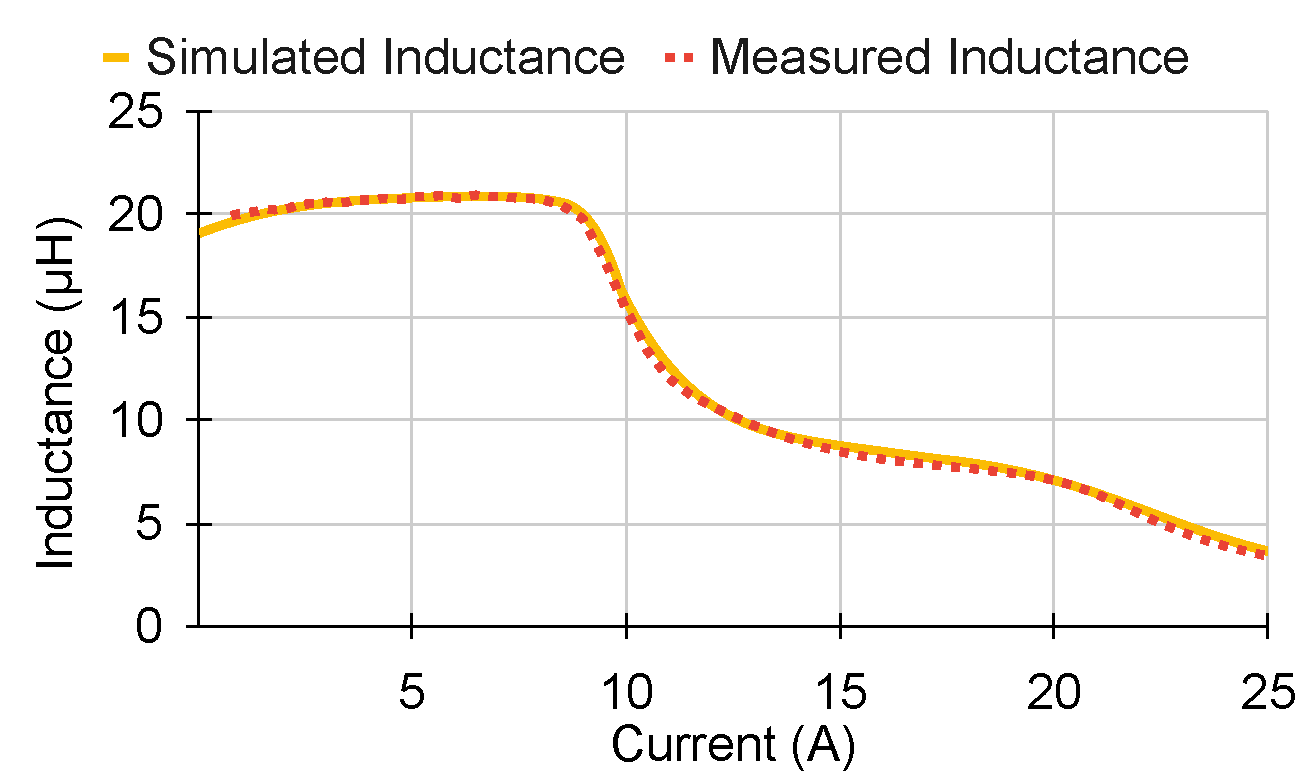
\includegraphics[width=0.7\linewidth]{Bilder/Kapitel3/Saturation_Measured_vs_LTspice.pdf}
    \caption{Comparison of the Inductance curve of the \textit{UA8014-AL} measured and simulated}
    \label{fig:comparison_of_saturation}
\end{figure}
\subsection{Validation by Ripple Current Amplitude}\label{sec:validation_by_ripple_current_amplitude}
To test the viability of the saturation model in a buck converter, the behaviour of its ripple current amplitude for different \ac{DC} bias currents is examined.\\

Simulating the inductor is done by connecting the model to a pulsing voltage source and constant current load. The voltage source simulates the excitation caused by the switching elements, without using direct \ac{GaNFET} models. This ensures that all effects are purely based on the inductor. To enable a ripple current to flow, a capacitor is also added in parallel to the current source, completing the circuit diagram shown here.
\begin{figure}[H]
    \centering
    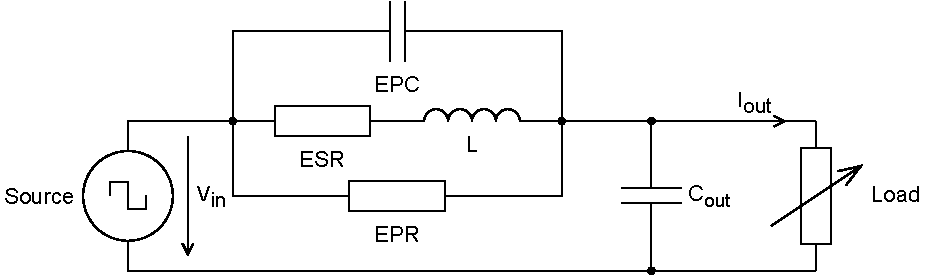
\includegraphics[width=1\linewidth]{Bilder/Kapitel4/Saturation_Validation_ECM.pdf}
    \caption{Circuit Diagram simulating the behaviour of a buck converter}
    \label{fig:saturation_validation_circuit_diagramm}
\end{figure}
The voltage source sends out rectangular voltage pulses with a 50\% duty cycle, \SI{30}{\V} peak at a switching frequency of \SI{300}{\kilo\Hz}. Measuring the peak-to-peak amplitude of the ripple current flowing through the \ac{ECM}, the current drawn by the simulated load is increased step by step from \SI{0.5}{\A} to \SI{20}{\A}. This process is then repeated for all five inductors. For the physical measurements, a buck converter with the same inductors is used. Its output current $I_{out}$ is also increased up to \SI{20}{A}.\\

Observing the measured data of the physical buck converter, a \ac{DC} dependent increase of the ripple currents amplitude is detected for all inductors. This increase, however, is not uniform between the inductors. For the \textit{SER1512} inductors, their ripple current scales up drastically, as soon as the approximate saturation current of \SI{7}{\A} and \SI{10}{\A} is reached. At \SI{20}{\A} \ac{DC} both register a peak-to-peak ripple current amplitude of more than \SI{15}{\A}. In comparison, the \textit{XGL1313} inductors only increase their ripple current amplitude slightly after reaching saturation.\\\\
\begin{figure}[h]
    \centering
    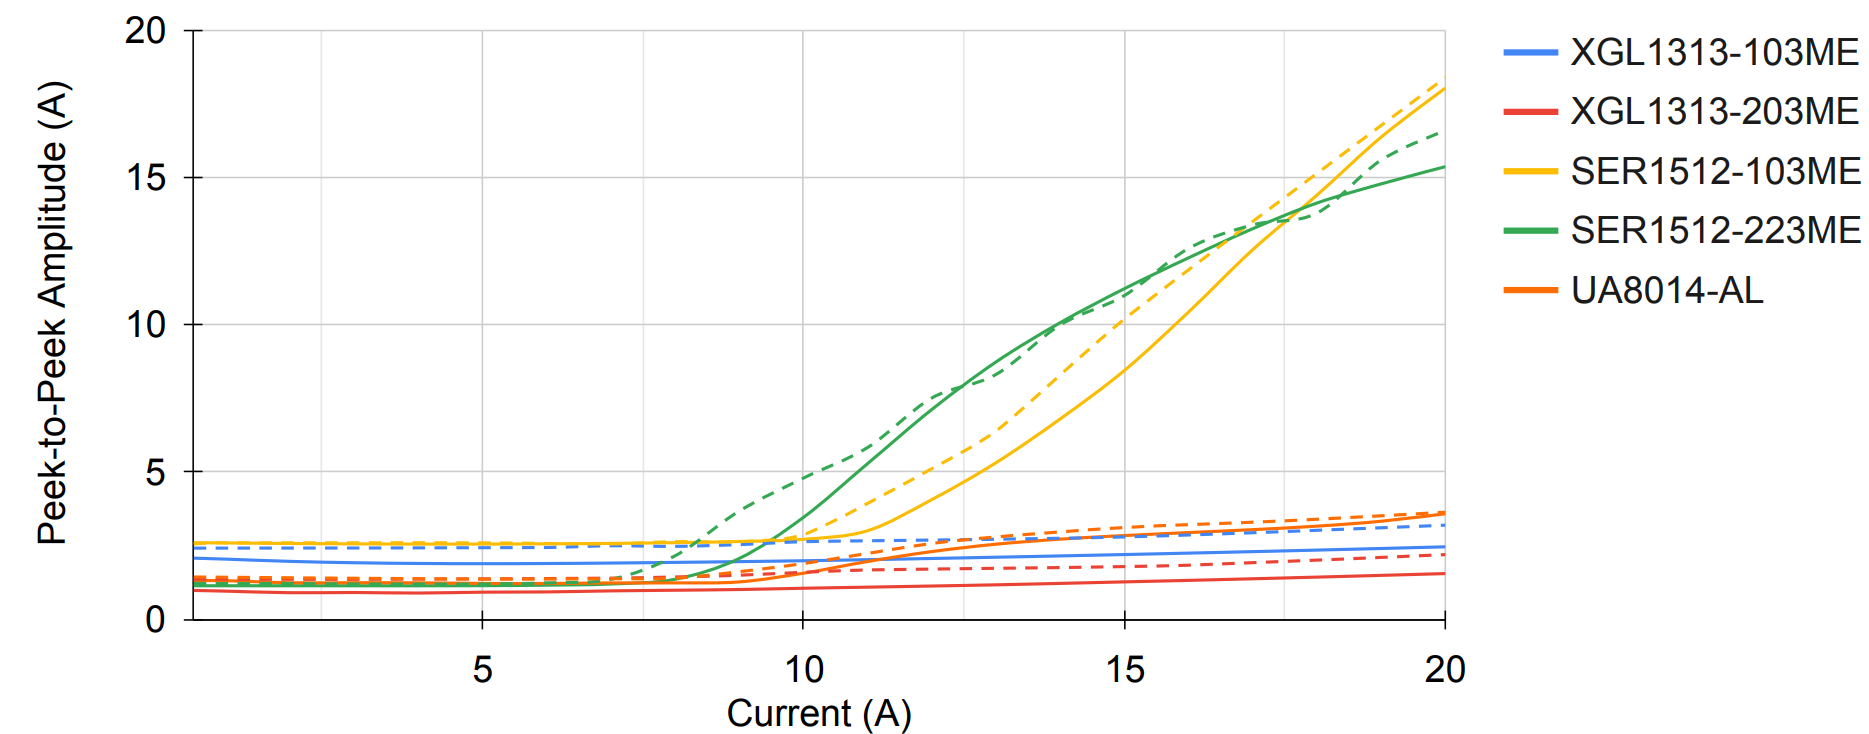
\includegraphics[width=1\linewidth]{Bilder//Kapitel4/High Current_2.png}
    \caption{Ripple current amplitude for high currents \\striped lines indicate measured values, while continuous lines are simulated}
    \label{fig:ripple_current_amplitude_for_high_currents}
\end{figure}
This behaviour mirrors the measured saturation curves. As seen in figure \ref{fig:comparison_of_saturation} the \textit{SER1512} experience a large inductance drop at saturation, while the \textit{XGL1313} gradually decrease their inductance due to a larger air gap. This causes the ripple current amplitude for a high \ac{DC} through the \textit{XGL1313} inductors, to not increase as drastically, as for the \textit{SER1512} inductors.\\\\
Regarding the simulated peak-to-peak amplitudes, their global behaviour reflects the behaviour of the real inductor well. For the inductors with a sharp inductance drop, their ripple current amplitude in the simulation increases rapidly too, while for the inductors with a gradual inductance decrease, their ripple current amplitude also increases gradually. While discrepancies are present, these are expected due to two main reasons. Firstly measurement errors in the peak-to-peak amplitudes of the physical buck converter introduce noise, most clearly seen for inductor \textit{SER1512-223ME}. Secondly, the saturation model is not able to represent the effects of \ac{DC} bias in the physical inductors. But even though this effect is not represented, the saturation model stays valid for both low currents, where saturation is not a factor, as well as high currents, where \ac{DC} bias has its greatest effect. \\

\section{Modeling the Hysteresis Behaviour of the Inductor}\label{modeling_the_hysteresis_behaviour_of_the_inductor}
The third type of LTspice inductor modelling examined is hysteresis modelling. In contrast to the saturation model, it takes the \ac{DC} bias into account with the hope of modelling the inductor behaviour at high output currents accurately.\\
In contrast to the flux, where a function can be directly input in LTspice, the hysteresis curve is defined via seven parameters: 
\begin{table}[H]
    \centering
    \caption{LTspice hysteresis modelling parameters}
    \begin{tabular}{|c|c|}
        \hline
        $N$ & Number of turns\\
        \hline
        $l_m$ & Length of magnetic core\\
        \hline
        $l_g$ & Length of air gap\\
        \hline
        $A_c$ & Crossectional area \\
        \hline
        $B_{max}$ & Maximum B-field\\
        \hline
        $B_r$ & Remnant B-field\\
        \hline
        $H_c$ & Coercivity\\
        \hline
    \end{tabular}
    \label{tab:ltspice_hystersis_modling_parameters}
\end{table}
To ensure that the use of ideal values in the LTspice simulation results in the desired behaviour and provides a representative model, the B-H curve is simulated purely with the values given by the cores data sheet, listed in table \ref{tab:parameters_of_the_custom_inductor} and table \ref{tab:B-H_curve_points_of_interest_comparison}. \\
Verifying the LTspice simulation is done by plotting the B-H curve of the simulated inductor. For this a sinusoidal current is applied to the inductor with no \ac{DC} bias and at the same frequency as the data sheet uses, \SI{10}{\kilo\Hz}. The B- and H-field values are calculated through Ampere's and Faraday's law given by equations \ref{eq:amperes_law_toH} and \ref{eq:faradays_law_toB}. \\
\begin{figure}[h]
    \centering
    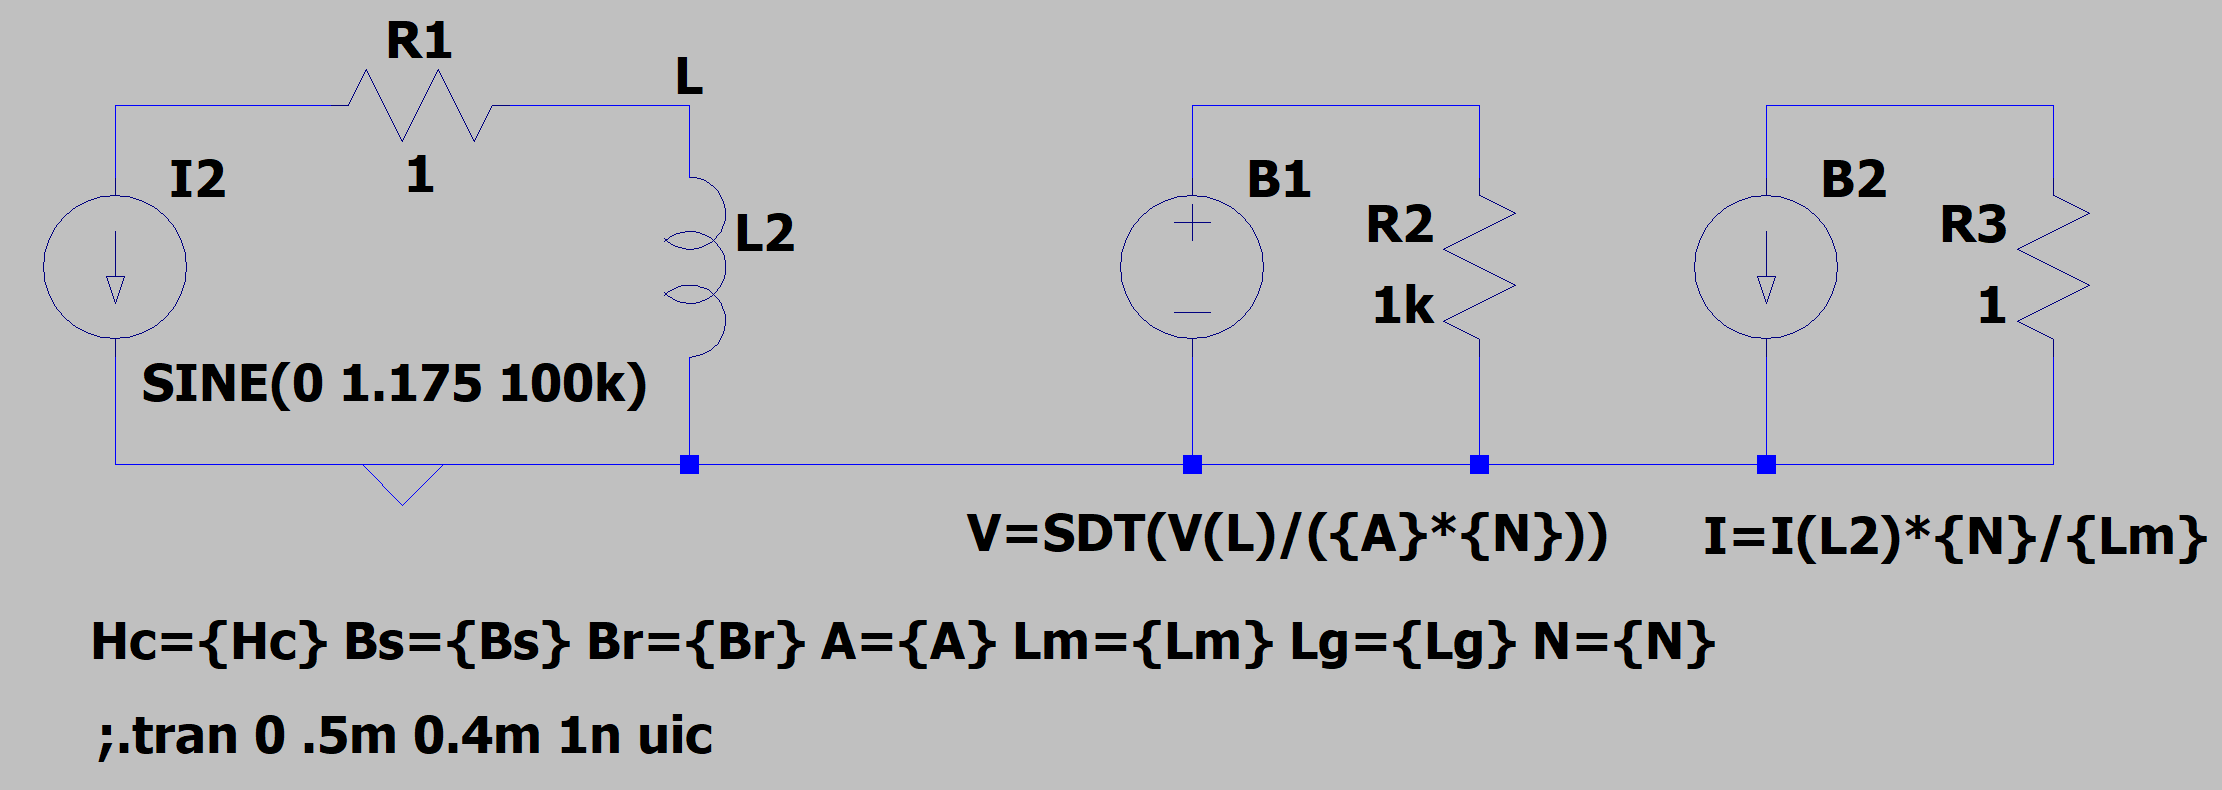
\includegraphics[width=.9\linewidth]{Bilder//Kapitel3/Hysteresis_Measurement_Setup_LTspice.png}
    \caption{Hysteresis measurement setup in LTspice}
    \label{fig:hysteresis_measurement_setup_in_LTspice}
\end{figure}
Using behavioural voltage and current sources, these equations are directly implemented in LTspice, as they allow for functions and integration.\\

Plotting the voltage of the behavioural voltage source versus the current of the behavioural current source yields the simulated B-H curve shown in figure \ref{fig:hysteresis_comparison}. The hysteresis behaviour is represented well in the simulation. While the maximum B-field $B_{max}$ does differ from the expected value by \SI{50}{\milli\tesla}, the remnant B-field $B_r$ and coercivity $H_c$ only differ minimally from the input values, by \SI{3}{\micro\tesla} and \SI{0.13}{\A\per\m} respectively.
\begin{figure}[H]
    \begin{subfigure}[b]{0.50\textwidth}
        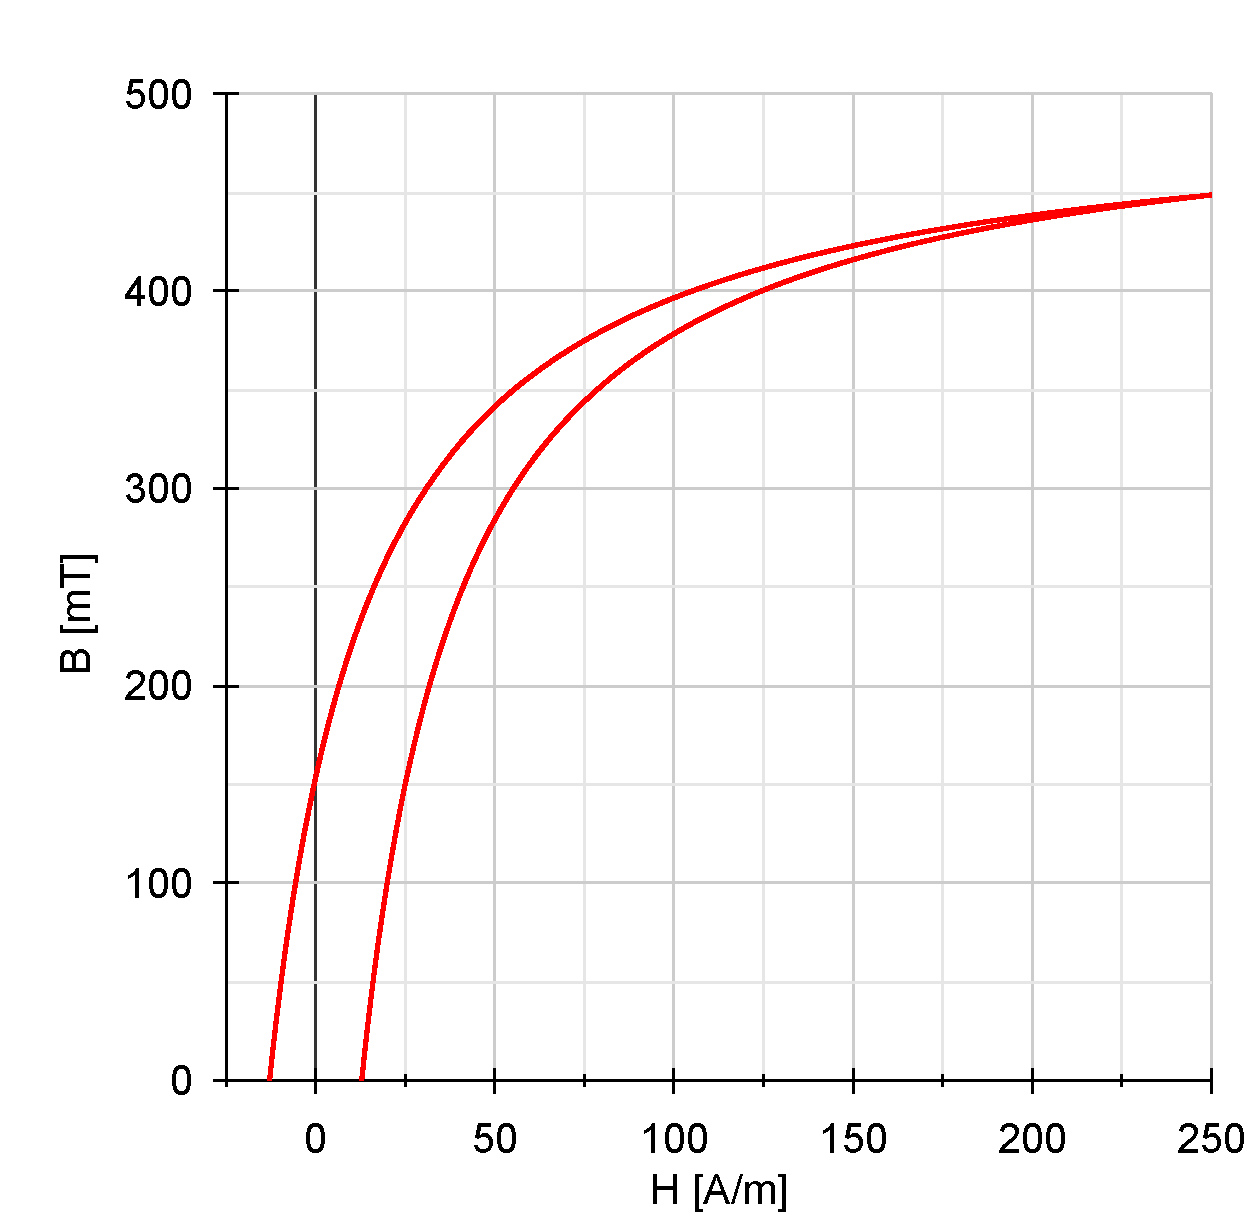
\includegraphics[width=\textwidth]{Bilder/Kapitel3/Hysteresis_LTspice_2.pdf}
        \caption{Simulated hysteresis curve}
    \end{subfigure}
    \begin{subfigure}[b]{0.49\textwidth}
        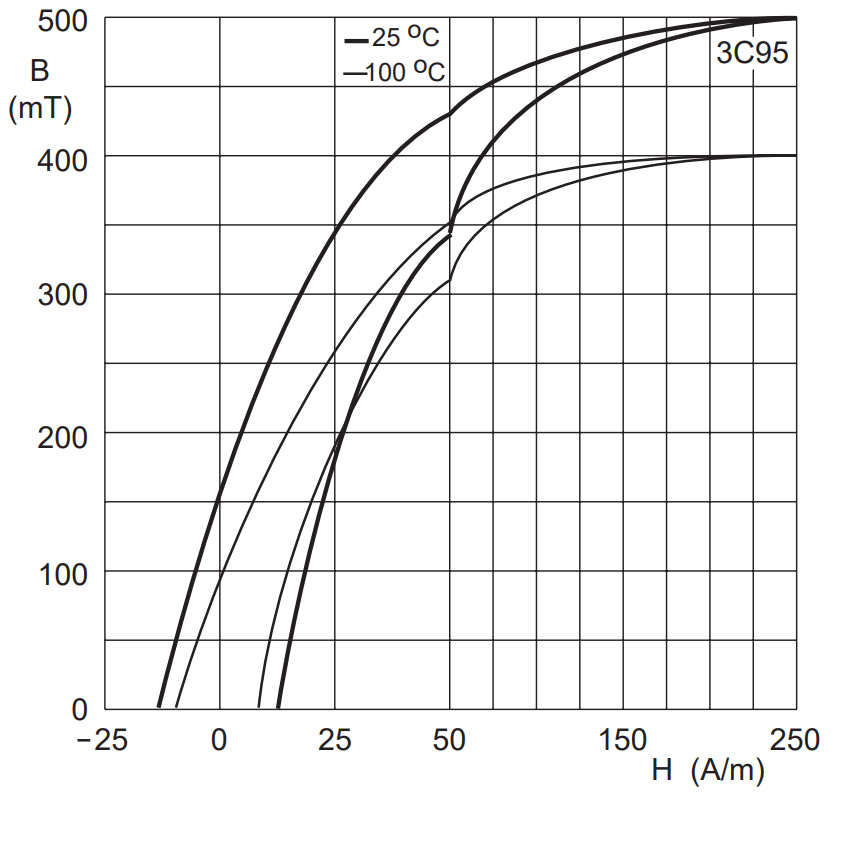
\includegraphics[width=\textwidth]{Bilder/Kapitel3/DataSheet_Hysteresis_Curve_2.png}
        \caption{Hysteresis given by the data sheet \cite{ferroxcubeProductSpecificationsCore2016}}
    \end{subfigure}
    \caption{Hysteresis comparison}
    \label{fig:hysteresis_comparison}							
\end{figure}
To validate the model's ability to function similarly to the model of section \ref{sec:modeling_the_saturation_behaviour_of_the_inductor} while adding the effects of \ac{DC} bias to the simulation, its saturation behaviour is examined. For this the measurement approach used in section \ref{sec:the_saturation_behaviour_of_the_inductor} is used again on the custom inductor. First, the physical inductor is measured and its saturation behaviour is extracted. Then the saturation of the simulated inductor model using the hysteresis parameters is measured. Their results are plotted in the graph \ref{fig:inductance_measured_and_simulatd}. 
\begin{figure}[H]
    \centering
    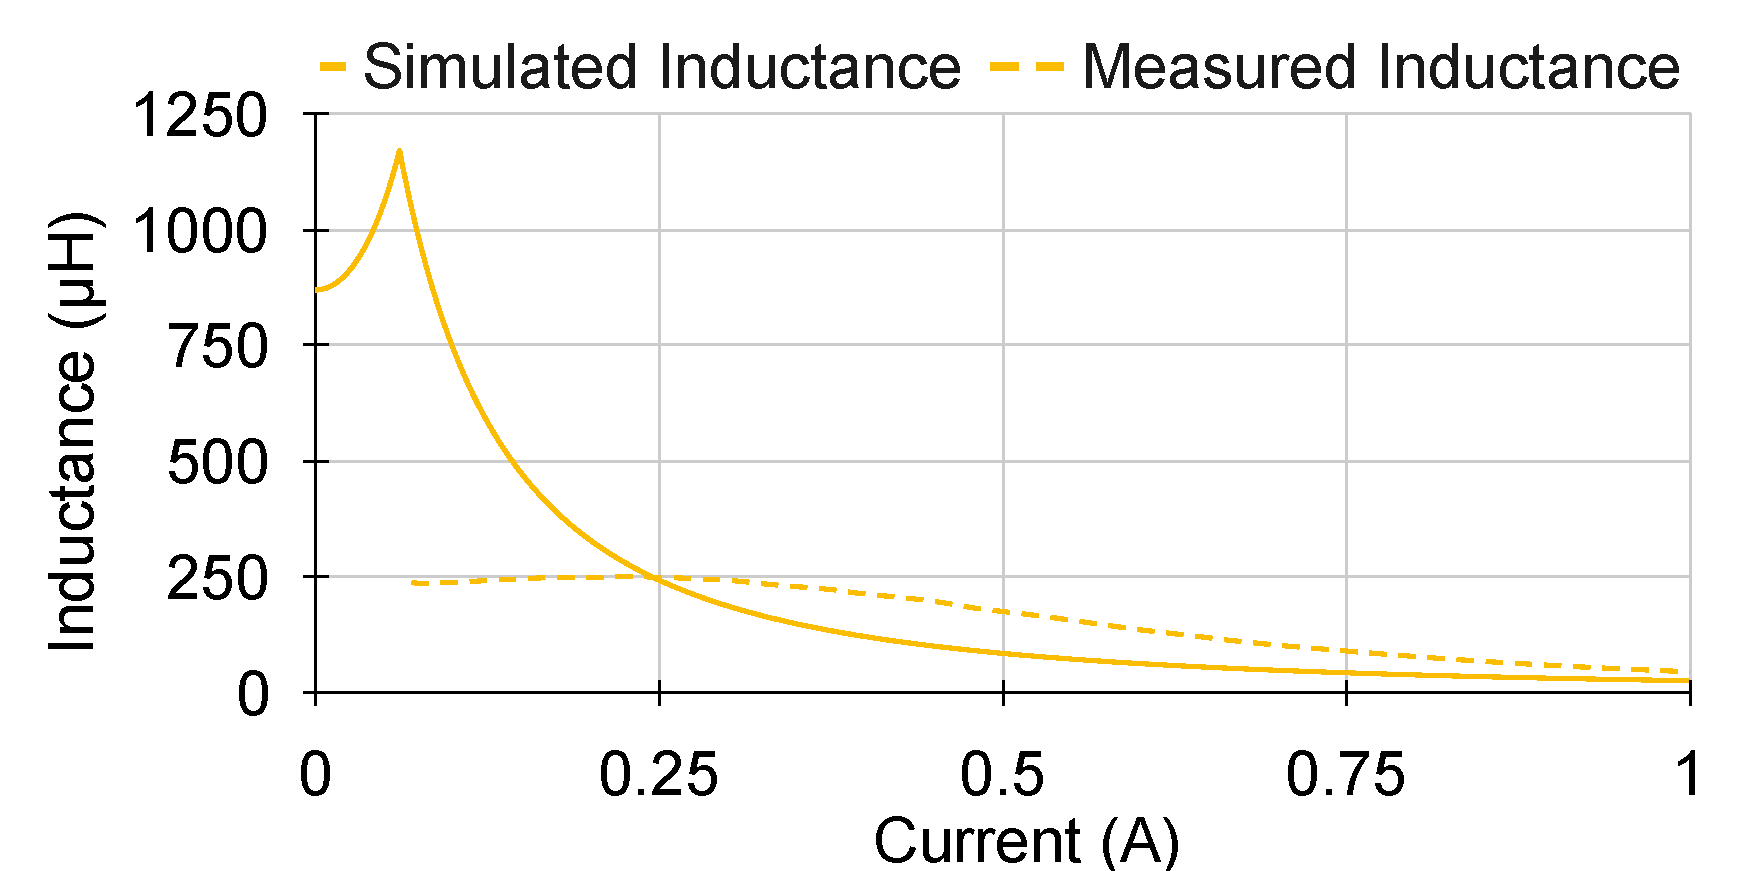
\includegraphics[width=.75\linewidth]{Bilder/Kapitel3/Saturation_Measured_and_Simulated_Hyst.pdf}
    \caption{Inductance measured and simulated}
    \label{fig:inductance_measured_and_simulatd}
\end{figure} 
Here the limits of the LTspice hysteresis modeling are shown. While demonstrating approximate hysteresis behaviour in figure \ref{fig:hysteresis_comparison}, the model is not able to recreate the inductance behaviour of the physical inductor, even though all measurement error from the hysteresis model has been removed.\\
Because of this, the hysteresis model is not implemented in the final inductor model.







